%************VERSUCHSANORDNUNG*************
\section{Experimental Setup}
\label{sec:versuchsandordnung}
The experimental work done in this thesis primarily utilized a Low-Temperature Scanning Tunneling Microscope setup.
This STM is composed of two distinct compartments, the preparation chamber (PC) the measurement chamber (MC).
The sample is inserted through a airlock into the preparation chamber.
In the whole system there is in a Ultra High Vacuum (UHV) at about 10$^{-11}$ - 10$^{-10}$ mbar, which is archieved by four individuall pumps.
The base Vacuum is achieved with the turbomolecular pump and the scroll pump through the airlock.
Additionally there is a titanium sublimation pump and a ion pump in the preparation room.

\monofig{width=\textwidth}{Experimental_Setup/STM_Picture_1_edited.pdf}{
    The experimental setup used, 
    A: cooling-chamber filled with Liquid Oxigen,
    B: measuring-chamber with spring suspended sample holder and tip,
    C: sputter-gun,
    D: metal-evaporater,
    E: molecule-evaporater,
    F: preparation-chamber with free movable sample holder arm,
    G: LEED system,
    H: Electronic used to monitor the function of the STM}{}
%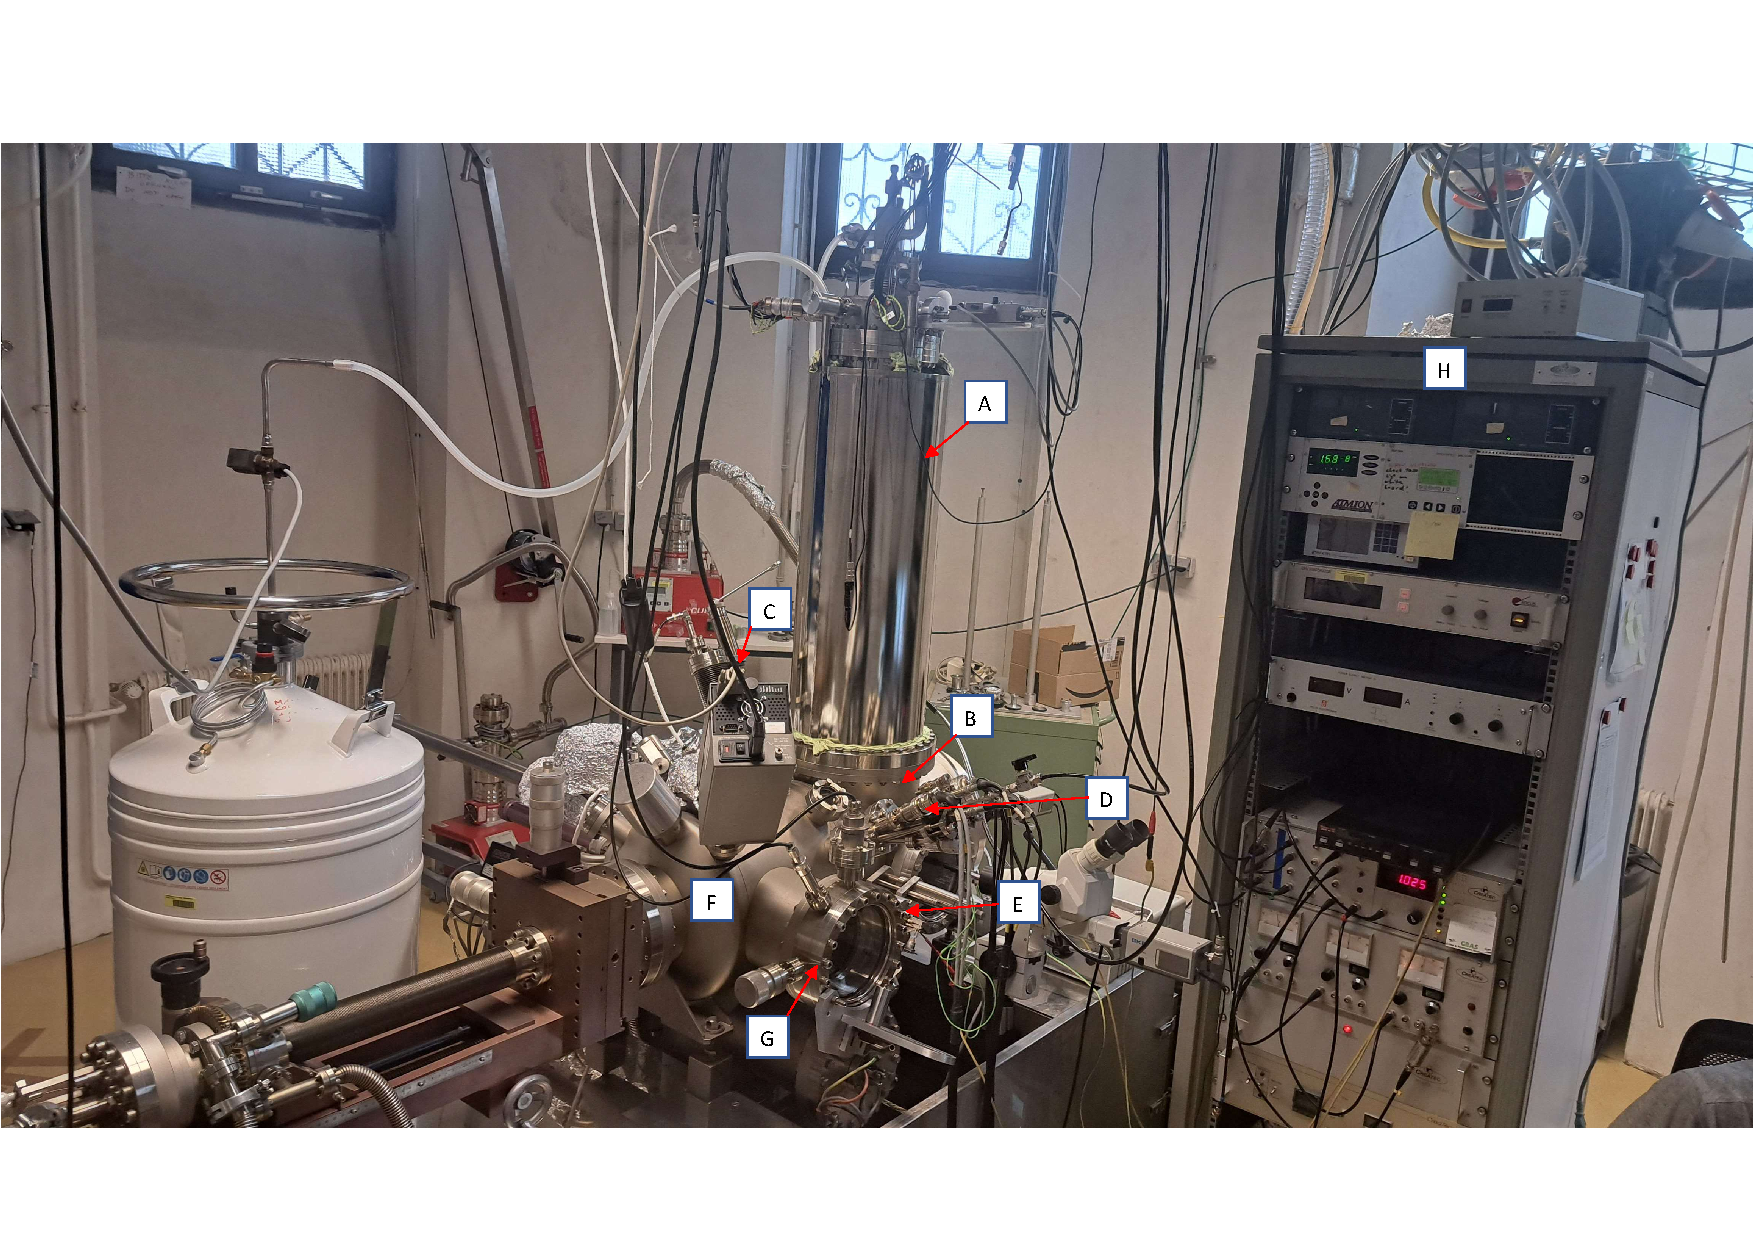
\includegraphics[width=0.9\textwidth]{Experimental_Setup/STM_Picture_1_edited.pdf}

The Probe-holder can be moved in each direction and rotated using an integrated arm in the PC.
It is also used to insert the Probe-holder into the MC.
The PC is equipped with a LEED system, which fluorescent screen can be extended 
At fixed positions in the PC there are ma